\section{Experiments}

The purpose of the experiments was to evaluate SEP on a number of datasets (synthetic and real-world, small and large) and on a number of models (probit regression, mixture of Gaussians for clustering, and Bayesian neural networks).

%%%% SECOND EXAMPLE %%%%
\subsection{Bayesian probit regression}
\label{sec:chap3_exp_bayesian_probit}
%
The first experiments considered a simple Bayesian classification problem and investigated the stability and quality of SEP in relation to EP and ADF as well as the effect of using mini-batches and varying the granularity of the approximation. The model comprised a probit likelihood function $P(\bm{y}_n = 1|\theta) = \Phi(\bm{\theta}^T \bm{x}_n)$ and a Gaussian prior over the hyper-plane parameter  $p(\bm{\theta}) = \mathcal{N}(\bm{\theta}; \bm{0}, \gamma I)$.  
%
The synthetic data comprised $N=5,000$ datapoints $\{ (\bm{x}_n, \bm{y}_n) \}$, where $\bm{x}_n$ were $D=4$ dimensional and were either sampled from a single Gaussian distribution (Fig.~\ref{fig:sep_probit}) or from a mixture of Gaussians (MoGs) with 5 components (Fig.~\ref{fig:daep_probit}) to investigate the sensitivity of the methods to the homogeneity of the dataset. The labels were produced by sampling from the generative model. We followed \cite{xu:sms2014} to measure the performance by computing an approximation of $\mathrm{KL}[p(\bm{\theta}|\mathcal{D}) || q(\bm{\theta})]$, where $p(\bm{\theta}|\mathcal{D})$ was replaced by a Gaussian that had the same mean and covariance as samples drawn from the posterior using the No-U-Turn sampler (NUTS) \citep{hoffman:nuts2014}. This evaluation metric measures how close the approximated first and second moments are to those of the exact posterior, and emphasises well calibrated uncertainty estimations.

Results in Fig.~\ref{fig:sep_probit} indicate that EP is the best performing method and that ADF collapses towards a delta function. SEP converges to a solution which appears to be of similar quality to that obtained by EP for the dataset containing Gaussian inputs, but slightly worse when the MoGs was used. Variants of SEP that used larger mini-batches fluctuated less, but typically took longer times to converge (although for the small mini-batches shown this effect is not clear). The utility of finer grained approximations depended on the homogeneity of the data. For the second dataset containing MoGs inputs (shown in Fig.~\ref{fig:daep_probit}), finer grained approximations were found to be advantageous if the datapoints from each mixture component are assigned to the same approximating factor. Generally it was found that there is no advantage to retaining more approximating factors than there were clusters in the dataset.  

Although not a main purpose, we further test the performance of SEP with sampling methods to compute moments (i.e.~SDEP).\footnote{code adjusted from \texttt{ep-stan}: \url{https://github.com/gelman/ep-stan}} We re-use the settings of probit regression but change the probit unit to sigmoid function, making the moment projection analytically intractable. We randomly partition the dataset into $J = 20$ subsets $\{\mathcal{D}_j\}$, construct the approximate posterior with local factors over the subsets, and tie them in SEP/AEP as before. Note that we perform sequential computations for DEP and AEP although they are ideally suited for parallel computing. Again as presented in Figure \ref{fig:sep_logit}, SEP performs almost as well as EP, which further justifies SEP even with sampling methods. Also AEP is indistinguishable from DEP, but it reduces memory by a factor of $N/J$.

To see if the trends carry to real-world datasets, we tested SEP's performance on six small binary classification datasets from the UCI machine learning repository.\footnote{\url{https://archive.ics.uci.edu/ml/index.html}} We did not consider the effect of mini-batches or the granularity of the approximation, using $J=M=1$. We ran the tests with damping and stopped learning after convergence (by monitoring the updates of approximating factors). The classification results are summarised in Table \ref{tab:chap3_sep_probit_results}. ADF performs reasonably well on the mean classification error metric, presumably because it tends to learn a good approximation to the posterior mode. However, the posterior variance is poorly approximated and therefore ADF returns poor test log-likelihood scores. EP achieves significantly higher test log-likelihood than ADF indicating that a superior approximation to the posterior variance is attained. Crucially, SEP performs very similarly to EP, implying that SEP is an accurate alternative to EP even though it is refining a cheaper global posterior approximation.

\begin{figure}
\centering
\subfigure[\label{fig:sep_probit}]{
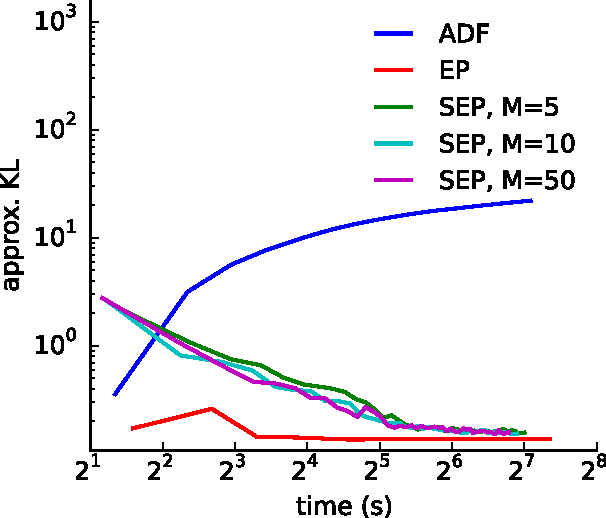
\includegraphics[width=0.30\linewidth]{Chapter3/sep/fig/sep_probit}}
%
\subfigure[\label{fig:daep_probit}]{
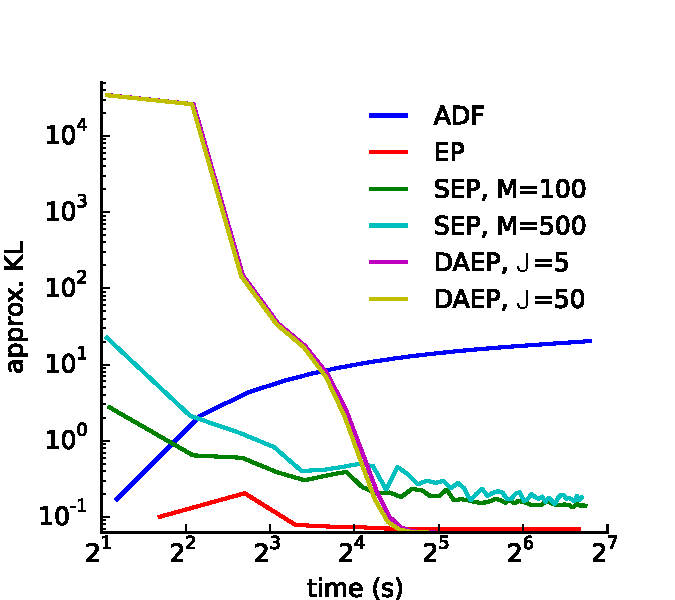
\includegraphics[width=0.35\linewidth]{Chapter3/sep/fig/daep.pdf}}
%
\subfigure[\label{fig:sep_logit}]{
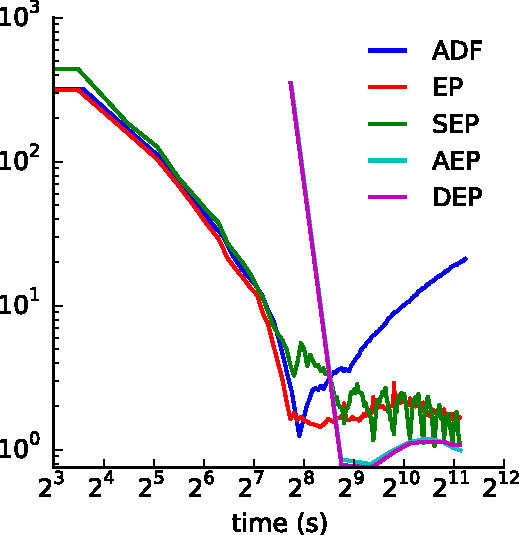
\includegraphics[width=0.26\linewidth]{Chapter3/sep/fig/sep_logit}}
\caption{Bayesian logistic regression experiments. Panels (a) and (b) show synthetic data experiments. Panel (c) shows the performance of EP-like methods on Bayesian logistic regression with the moment matching step computed by NUTS. $M$ denotes the mini-batch size for data sub-sampling (may be within a data piece for panel (c)). EP (in red curves) is the best performing method in terms of the approximate KL metric.  SEP works slightly worse but with its performance approaching to EP as the running time grows. ADF over-counts the number of observations and thus returns worst results as expected.}
\end{figure}

\begin{table} 
\small
\centering
 \caption{ Average test results all methods on probit regression (mean and standard error reported). All methods capture a good posterior mode, however EP outperforms ADF in terms of test log-likelihood on almost all the datasets, with SEP performing similarly to EP.}
  \label{tab:chap3_sep_probit_results} 
  \scalebox{0.9}{
\begin{tabular}{l@{\ica}r@{$\pm$}l@{\ica}r@{$\pm$}l@{\ica}r@{$\pm$}l | @{\ica}r@{$\pm$}l@{\ica}r@{$\pm$}
	l@{\ica}r@{$\pm$}l@{\ica}r@{$\pm$}}\hline 
{} & \multicolumn{6}{c}{mean error} & \multicolumn{6}{c}{test log-likelihood} \\
\bf{Dataset}&\multicolumn{2}{c}{\bf{ ADF }}&\multicolumn{2}{c}{\bf{ SEP }}&\multicolumn{2}{c}{\bf{ EP }} &\multicolumn{2}{c}{\bf{ ADF }}&\multicolumn{2}{c}{\bf{ SEP }}&\multicolumn{2}{c}{\bf{ EP }} \\ \hline 
%
Australian&0.328&0.0127&\bf{0.325}&\bf{0.0135}&0.330&0.0133
	&-0.634&0.010&\bf{-0.631}&\bf{0.009}&\bf{-0.631}&\bf{0.009}\\
%
Breast&0.037&0.0045&\bf{0.034}&\bf{0.0034}&\bf{0.034}&\bf{0.0039}
	&-0.100&0.015&-0.094&0.011&\bf{-0.093}&\bf{0.011}\\
%
% Crabs results after convergence
Crabs&0.056&0.0133&\bf{0.033}&\bf{0.0099}&0.036&0.0113
	&-0.242&0.012&-0.125&0.013&\bf{-0.110}&\bf{0.013}\\
% Crabs results for only 40 iterations (not converged)
%Crabs&0.062&0.0125&\bf{0.040}&\bf{0.0106}&0.048&0.0117
%	&-0.290&0.010&\bf{-0.177}&\bf{0.012}&-0.217&0.011\\
%
Ionos&\bf{0.126}&\bf{0.0166}&0.130&0.0147&0.131&0.0149
	&-0.373&0.047&-0.336&0.029&\bf{-0.324}&\bf{0.028}\\
%
Pima&0.242&0.0093&0.244&0.0098&\bf{0.241}&\bf{0.0093}
	&-0.516&0.013&-0.514&0.012&\bf{-0.513}&\bf{0.012}\\
%
Sonar&\bf{0.198}&\bf{0.0208}&\bf{0.198}&\bf{0.0217}&\bf{0.198}&\bf{0.0243}
	&-0.461&0.053&-0.418&0.021&\bf{-0.415}&\bf{0.021}\\
 \hline \end{tabular} }
 \end{table} 
 
\subsection{DSEP experiments and grouping tests}

The assumption we made in the main text to achieve SEP $\approx$ full EP is that the contributions of each likelihood term to the posterior are very similar. We show further results here on the approximation produced by different EP methods when we believe there exists heterogeneity in data.
%
We generated synthetic XOR classification data by sampling from 4 unit Gaussians with means $(3, 3)$, $(-3, -3)$, $(3, -3)$ and $(-3, 3)$, and labelling the clusters centred at the former two as negative examples (and positive for the others). The model $p(y_n|\bm{x}_n, \bm{\theta})$ is kernel probit regression using RBF kernel with width $l=1.0$, which is the same as the model presented in Section \ref{sec:chap3_exp_bayesian_probit} except that the features are changed to kernel representations. This makes the feature vectors high dimensional, and the local nature of kernels also makes them very different if the datapoints belong to different clusters. We generated $50 \times 4$ test data and $\{10 \times 4, 20 \times 4, 50 \times 4\}$ training data and ran SEP/DSEP/full EP to approximate the posterior distribution of $\bm{\theta}$. For DSEP we partitioned the dataset into 4 subsets according to the associated centroid. Each experiment was repeated 10 times to collect average test data log-likelihood and classification error.

Table \ref{tab:kernel} shows the quantitative numbers of performances and Figure \ref{fig:kernel_increase_n} visualises the contours of probability $p(y = 1|\bm{x}, \mathcal{D})$ with true posterior approximated by $q(\bm{\theta})$. Interestingly SEP is slightly better then the others on the classification error metric. But importantly EP achieves the best test log-likelihood numbers and in general DSEP produces very similar results (shown by both the table and the figure), meaning that even for small datasets running full EP might be unnecessary. Also the three methods become indistinguishable when the size of the dataset $N$ increases. We argue the main reason is that the posterior contributions are getting similar since more datapoints are observed in the circle of kernel width.

We further tested the robustness of all three methods to outliers. We reused the settings above and randomly flipped $10\%$ labels of training data. Qualitative results in Figure \ref{fig:kernel_flip} show that SEP is almost as robust as DSEP/EP in this example. We had tried different types of outliers and failed to find the cases where EP/DSEP significantly outperforms SEP. Future work should answer the questions that when SEP gives bad approximations and whether it fails in the same way as EP fails.


\begin{table} 
\small
\centering
 \caption{ Average test results of all methods on kernel probit regression.}
  \label{tab:kernel} 
  \scalebox{0.9}{
\begin{tabular}{l@{\ica}r@{$\pm$}l@{\ica}r@{$\pm$}l@{\ica}r@{$\pm$}l@{\ica}r@{$\pm$}l@{\ica}r@{$\pm$}
	l@{\ica}r@{$\pm$}l@{\ica}r@{$\pm$}}\hline 
{} & \multicolumn{6}{c}{mean error} & \multicolumn{6}{c}{test log-likelihood} \\
\bf{$N$}&\multicolumn{2}{c}{\bf{ SEP }}&\multicolumn{2}{c}{\bf{ DSEP }}&\multicolumn{2}{c}{\bf{ EP }} &\multicolumn{2}{c}{\bf{ SEP }}&\multicolumn{2}{c}{\bf{ DSEP }}&\multicolumn{2}{c}{\bf{ EP }} \\ \hline 
%
$10 \times 4$&\bf{0.032}&\bf{0.0058}&0.055&0.0127&\bf{0.032}&\bf{0.0097} 
	&-0.405&0.011&-0.380&0.010&\bf{-0.378}&\bf{0.009} \\
%
$20 \times 4$&\bf{0.007}&\bf{0.0014}&0.008&0.0024&0.012&0.0031 
	&-0.326&0.007&-0.320&0.006&\bf{-0.317}&\bf{0.003} \\
%
$50 \times 4$&\bf{0.003}&\bf{0.0010}&\bf{0.003}&\bf{0.0014}&0.006&0.0009 
	&-0.243&0.004&\bf{-0.233}&\bf{0.007}&-0.238&0.003 \\
%
 \hline \end{tabular} }
 \end{table} 

\begin{figure}
\centering
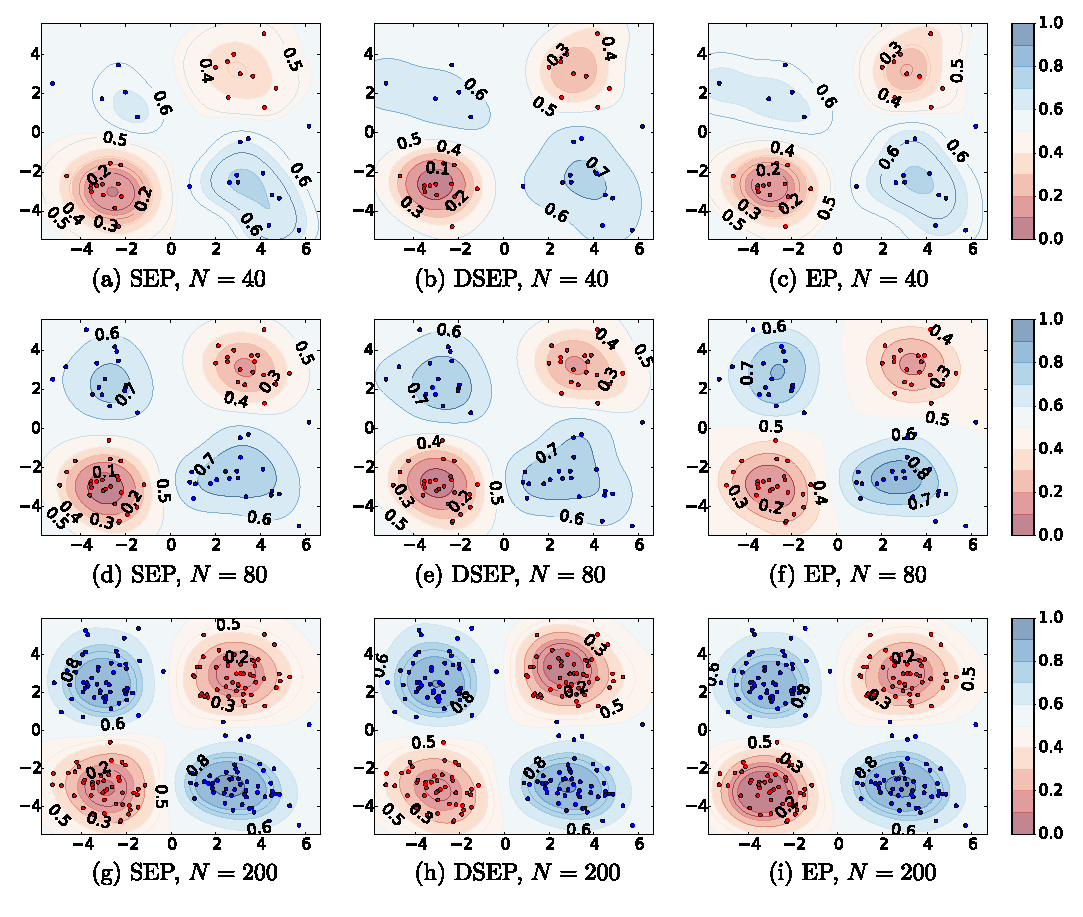
\includegraphics[width=1\linewidth]{Chapter3/sep/fig/increase_n_kernel}
\caption{Comparing predictions of kernel Probit regression trained by SEP/DSEP/EP, with increasing training data size $N$. Although not very significant, for $N=40$ the decision boundary obtained by the DSEP method is more similar to that of the full-EP method. This difference vanishes as $N$ increases. }
\label{fig:kernel_increase_n}
\end{figure}

\begin{figure}
\centering
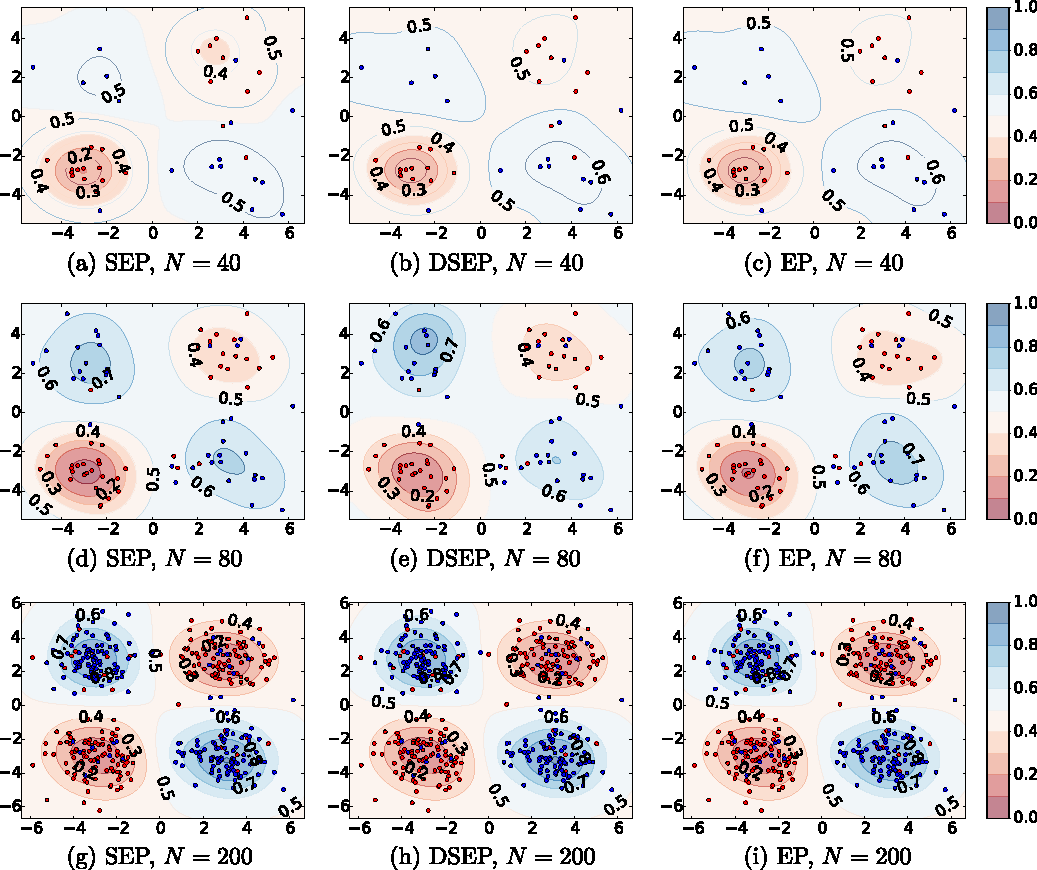
\includegraphics[width=1\linewidth]{Chapter3/sep/fig/flip_kernel}
\caption{Comparing predictions of kernel probit regression trained by SEP/DSEP/EP, with $10\%$ labels flipped. The same observations as to the results in \ref{fig:kernel_increase_n} apply.}
\label{fig:kernel_flip}
\end{figure}

To verify whether these conclusions about the granularity of the approximation hold in real datasets, we sampled $N=1,000$ datapoints for each of the digits in MNIST and performed odd-vs-even classification. Each digit class was assigned its own global approximating factor, $J=10$. We compare the log-likelihood of a test set using ADF, SEP ($J=1$), full EP and DSEP ($J=10$) in Figure \ref{fig:mnist}. EP and DSEP significantly outperform ADF. DSEP is slightly worse than full EP initially, however it reduces the memory to 0.001\% of full EP without losing substantial accuracy. SEP's accuracy was still increasing at the end of learning and was slightly better than ADF.

\begin{figure}
\centering
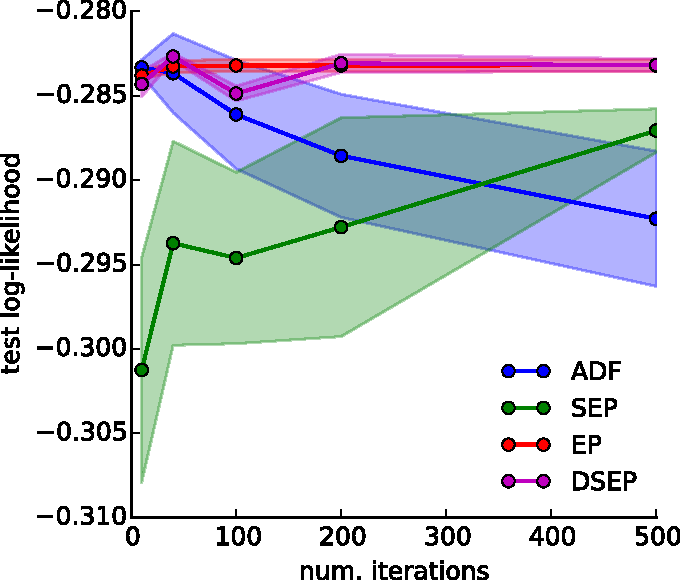
\includegraphics[width=0.4\linewidth]{Chapter3/sep/fig/mnist_error}
\caption{DSEP experimental result on MNIST (mean and standard error reported, see text for full details).}
\label{fig:mnist}
\end{figure} 
 
 %
%%%% FIRST EXAMPLE %%%%
\subsubsection{Mixture of Gaussians for clustering}
%
The small scale experiments on probit regression indicate that SEP performs well for fully-observed probabilistic models. Although it is not the main focus of the section, we sought to test the flexibility of the method by applying it to a latent variable model, specifically a mixture of Gaussians (MoGs). A synthetic MoGs dataset containing $N=200$ datapoints was constructed comprising 4 Gaussians. The means were sampled from a Gaussian distribution, $p(\bm{\mu}_j)= \mathcal{N}(\bm{\mu}; \bm{m}, \mathbf{I})$, the cluster identity variables $\bm{h}_n$ were sampled from a uniform categorical distribution, and each mixture component was isotropic $p(\bm{x}_n | \bm{h}_n) = \mathcal{N}(\bm{x}_n; \bm{\mu}_{\bm{h}_n}, 0.5^2 \mathbf{I})$. EP, ADF and SEP were performed to approximate the joint posterior over the cluster means $\{ \bm{\mu}_j\}$ and cluster identity variables $\{ \bm{h}_n \}$ (the other parameters were assumed known). 

Figure \ref{fig:gmm_visualised} visualises the approximate posteriors after 200 iterations. All methods return good estimates for the means, but ADF collapses towards a point estimate as expected. SEP, in contrast, captures the uncertainty and returns nearly identical approximations to EP. The accuracy of the methods is quantified in Fig.~\ref{fig:gmm_error} by comparing the approximate posteriors to those obtained from NUTS. In this case the approximate KL-divergence measure is analytically intractable, instead we used the averaged Frobenius-norm (F-norm) of the difference of the Gaussian parameters fitted by NUTS and EP methods. These measures confirm that SEP approximates EP well.

\begin{figure}
\centering
\subfigure[\label{fig:gmm_visualised}]{
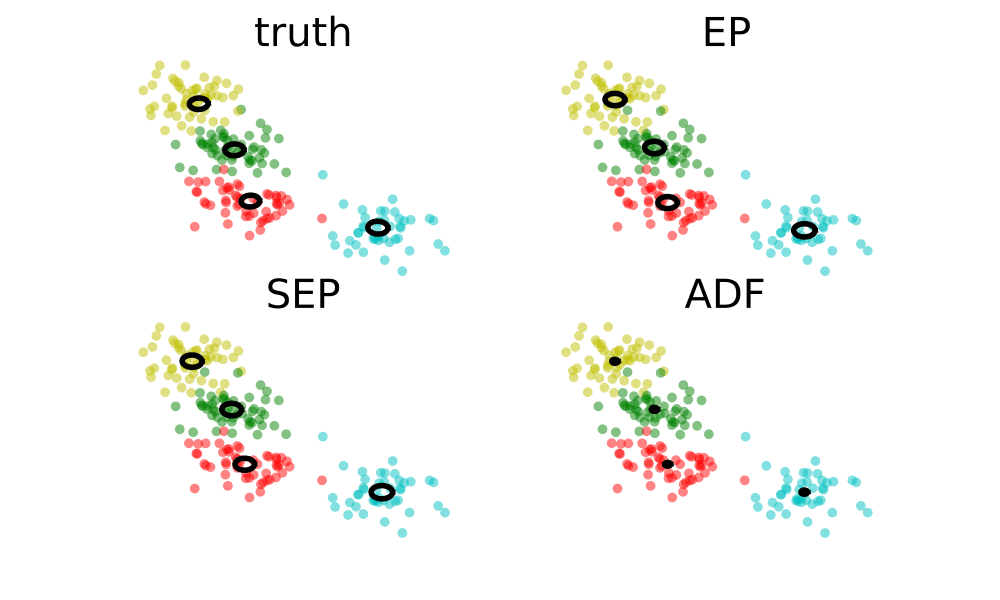
\includegraphics[width=0.5\linewidth]{Chapter3/sep/fig/gmm1.png}}
%
\hspace{0.1in}
%
\subfigure[\label{fig:gmm_error}]{
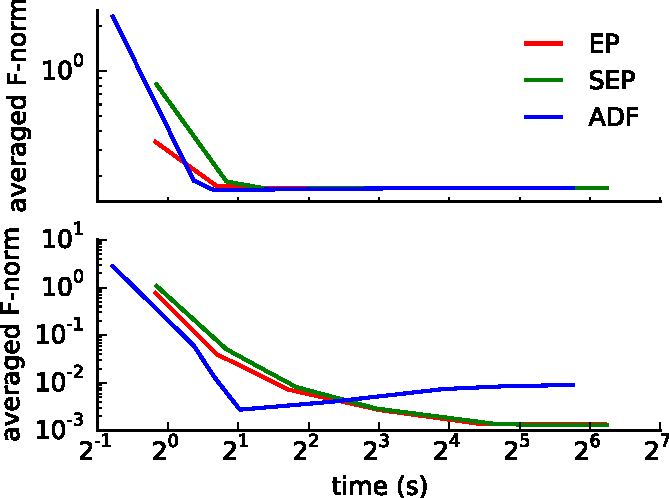
\includegraphics[width=0.42\linewidth]{Chapter3/sep/fig/gmm_error}}
\caption{Posterior approximation for the mean of the Gaussian components. (a) visualises posterior approximations over the cluster means (98\% confidence level). The coloured dots indicate the true label (top-left) or the inferred cluster assignments (the rest). In (b) we show the error (in F-norm) of the approximate Gaussians' means (top) and covariances (bottom). }
\end{figure}

\subsection{Probabilistic back-propagation for Bayesian neural nets}

The final set of tests consider more complicated models and large datasets. Specifically we evaluate the methods for probabilistic back-propagation (PBP) \citep{hernandez-lobato:pbp2015}, a
recent state-of-the-art method for scalable Bayesian learning in neural
network models.\footnote{See Appendix \ref{sec:appendix_pbp} for detailed update equations.} Previous implementations of PBP perform several iterations of ADF over the training
data. The moment-matching operations required by ADF are themselves intractable and they are approximated by first propagating the uncertainty on the synaptic weights forward through the network in a sequential way, 
and then computing the gradient of the marginal likelihood by back-propagation.
Previous implementations of PBP are based on ADF to reduce the large memory cost that would be required by EP when the amount of available data is very large.

We performed neural network regression experiments with publicly available data sets and neural networks with one hidden layer.  Table~\ref{tab:chap3_sep_datasets_neural_networks} lists the analysed data sets and shows summary statistics.  We used neural networks with 50 hidden units in all cases except in the two largest ones, i.e., \emph{Year Prediction
MSD} and \emph{Protein Structure}, where we used 100 hidden units. The different methods, SEP, EP and ADF were run by performing 40 passes over the available training data, updating the parameters of the posterior approximation after seeing each data point.  The data sets were split into random training and test sets with 90\% and 10\% of the data, respectively. This splitting process was repeated 20 times for the small datasets, and the average test performances of each method were reported. In the two largest data sets, \emph{Year Prediction MSD} and \emph{Protein Structure}, we did the train-test splitting only one and five times respectively. The datasets were normalised so that the input features and the targets have zero mean and unit variance in the training set. The normalisation on the targets was removed for prediction.

Table \ref{tab:chap3_sep_pbp_results} shows the average test RMSE and test log-likelihood for each method. Interestingly, SEP can outperform EP in this setting (possibly because the stochasticity enabled it to find better solutions), and typically it performed similarly. Surprisingly ADF often outperformed EP, although the results presented for ADF use a near-optimal number of sweeps and further iterations generally degraded performance. ADF's good performance is most likely due to an interaction with additional the moment-approximation that is required in PBP.

\begin{table} 
\small
\centering 
\caption{Average test results for all methods on Bayesian neural networks (mean and standard error reported). Datasets are also from the UCI machine learning repository.} 
\label{tab:chap3_sep_pbp_results} 
\scalebox{0.9}{
\begin{tabular}{l@{\ica}r@{$\pm$}l@{\ica}r@{$\pm$}l@{\ica}r@{$\pm$}l | @{\ica}r@{$\pm$}l@{\ica}r@{$\pm$}l@{\ica}r@{$\pm$}l@{\ica}r@{$\pm$}}\hline 
{} & \multicolumn{6}{c}{RMSE} & \multicolumn{6}{c}{test log-likelihood} \\
\bf{Dataset}&\multicolumn{2}{c}{\bf{ ADF }}&\multicolumn{2}{c}{\bf{ SEP }}&\multicolumn{2}{c}{\bf{ EP }} &\multicolumn{2}{c}{\bf{ ADF }}&\multicolumn{2}{c}{\bf{ SEP }}&\multicolumn{2}{c}{\bf{ EP }} \\ \hline 
%
Kin8nm&0.098&0.0007&\bf{0.088}&\bf{0.0009}&0.089&0.0006
	&0.896&0.006&\bf{1.013}&\bf{0.011}&1.005&0.007\\ 
%
Naval&0.006&0.0000&\bf{0.002}&\bf{0.0000}&0.004&0.0000
	&3.731&0.006&\bf{4.590}&\bf{0.014}&4.207&0.011\\  
%
Power&\bf{4.124}&\bf{0.0345}&4.165&0.0336&4.191&0.0349
	&\bf{-2.837}&\bf{0.009}&-2.846&0.008&-2.852&0.008\\
% 
Protein&4.727&0.0112&\bf{4.670}&\bf{0.0109}&4.748&0.0137
	&-2.973&0.003&\bf{-2.961}&\bf{0.003}&-2.979&0.003\\ 
%
Wine&\bf{0.635}&\bf{0.0079}&0.650&0.0082&0.637&0.0076
	&-0.968&0.014&-0.976&0.013&\bf{-0.958}&\bf{0.011}\\  
%
Year&\bf{8.879}&\bf{   NA}&8.922&   NA&8.914&   NA
&\bf{-3.603}&\bf{  NA}&-3.924&  NA&-3.929&  NA\\
 \hline \end{tabular} }
 \end{table} 


We also provide the memory consumption details for experiments using PBP in Table \ref{tab:chap3_sep_datasets_neural_networks}, where some of the results are also visualised in Figure \ref{fig:chap3_sep_memory_saving}. We observe substantial memory reductions by running SEP instead of EP, while still attaining similar accuracies. Especially for Year Prediction MSD dataset, which is a typical large-scale dataset both in the number of observations $N$ and the dimensionality $D$, SEP achieves tens of gigabytes savings.\footnote{In this case we used mean-field Gaussian approximations, meaning that a Gaussian factor costs $\mathcal{O}(HD)$ storage with $H=50$ the number of hidden units.} We performed the test for EP using a machine with more than 100GB RAM, while SEP only required 2.7GB memory, including the space of storing the dataset (roughly 1.9GB). These numbers reveal the huge memory requirement of full EP and further support SEP as a practical alternative in big data, big model settings.

To summarise, in all the experiments presented in this section, we observed that SEP performed almost equally well as full EP, and at the same time provided substantial memory complexity gains. By noticing that the posterior only cares about the product of the likelihood terms, we conjecture that, whilst SEP provides worse approximations to individual likelihood terms, it approximates the product of the product of the likelihood terms almost as well as the full EP case. This again justifies the motivation of SEP that it focuses only on the approximation to the ``averaged likelihood'', and full EP, which considering accurate approximations to each individuals, might seem like an over-kill in practice.

\begin{table} 
\caption{Datasets used in the experiments with neural networks. The memory figures reported include dataset storage and temporal maintenance of computation graphs in Theano \citep{Bastien-Theano-2012} ($\sim100MB$ for small datasets and $\sim 1.9GB$ for Year Prediction MSD).}
\label{tab:chap3_sep_datasets_neural_networks} 
\centering 
\begin{tabular}{lrrrrr} 
\hline  
\textbf{Dataset} & $N$ & $D$ & MB (EP) & MB (SEP) & MB reduced \tabularnewline 
\hline 
Kin8nm & 8192 & 8 & 168.23 & 109.76 & 58.47 \tabularnewline 
Naval Propulsion & 11,934 & 16 & 261.75 & 113.92 & 147.83 \tabularnewline 
Combined Cycle Power Plant & 9568 & 4 & 148.70 & 110.99 & 37.71 \tabularnewline 
Protein Structure & 45,730 & 9 & 815.55 & 121.52 & 694.02 \tabularnewline 
Wine Quality Red & 1599 & 11 & 122.21 & 107.90 & 14.30 \tabularnewline 
\bf{Year Prediction MSD} & \bf{515,345} & \bf{90} & \bf{67837.90} & \bf{2730.55} & \bf{65107.34} \tabularnewline 
\hline 
\end{tabular}
\end{table}

\begin{figure}
\centering
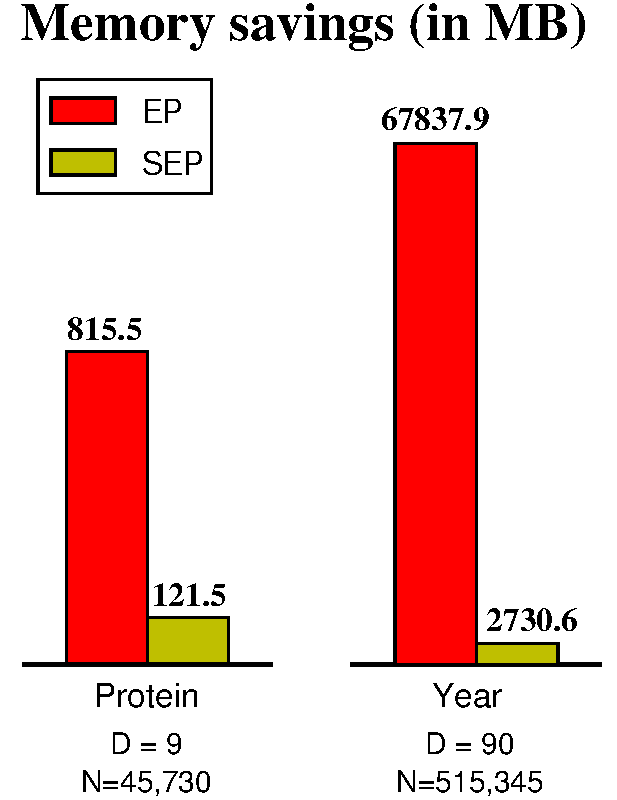
\includegraphics[width=0.4\linewidth]{Chapter3/sep/fig/memory_saving}
\caption{A visualisation of storage savings by SEP.}
\label{fig:chap3_sep_memory_saving}
\end{figure}
